\section{Preprocessing}
\label{sec:preprocessing}

La fase di preprocessing ha l'obiettivo di rendere il modello CAD quanto più consistente possibile, prima che venga elaborato dal resto della pipeline. Si interviene correggendo manualmente i nomi di layer e blocchi, e riparando eventuali geometrie incomplete o ridondanti.

Come caso di studio si considera il seguente modello CAD, aperto in LibreCAD per una prima analisi (Figura ~\ref{fig:caso_studio}). 
\begin{figure}[htbp]
	\centering
	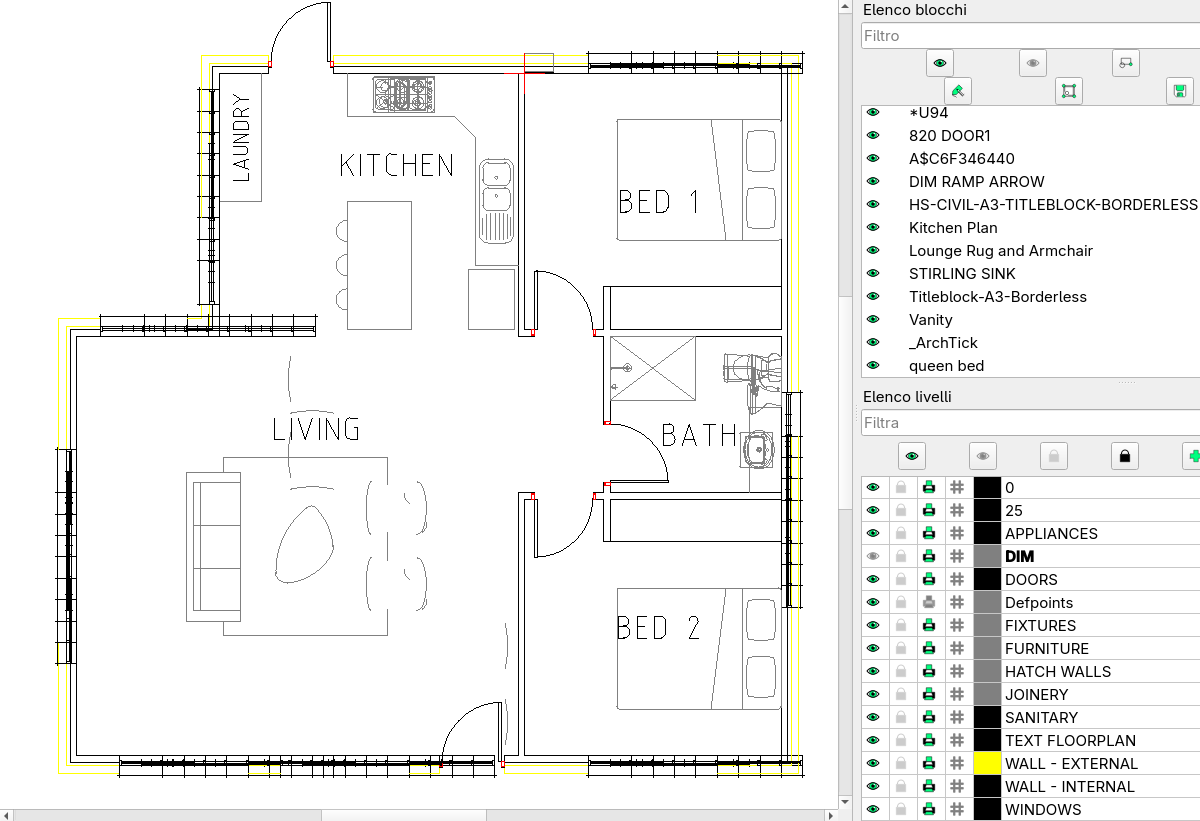
\includegraphics[width=1\textwidth]{figures/3_progettazione_pipeline/caso-studio.png}
	\caption{Modello CAD del caso di studio aperto in LibreCAD: sono visibili i layer e i blocchi con denominazioni non conformi ai criteri imposti.}
	\label{fig:caso_studio}
\end{figure}

Un primo problema riguarda la denominazione di layer e blocchi, che non rispetta la convenzione imposta nella Sezione \ref{sec:assunzioni_progettuali}; è quindi necessario rinominarli secondo i criteri richiesti.

Il modello presenta inoltre sia muri interni (layer \texttt{WALL-INTERNAL}) sia muri esterni (layer \texttt{WALL-EXTERNAL}). Questi ultimi risultano ridondanti e possono essere rimossi senza alcun impatto sulla geometria finale. Isolando i muri, si osserva come la loro geometria risulti "spezzata": i contorni formano poligoni aperti, in violazione delle condizioni di validità imposte nella Sezione \ref{sec:assunzioni_progettuali}, e richiedono pertanto una correzione manuale (Figura ~\ref{fig:muri_rotti}).
\begin{figure}[htbp]
	\centering
	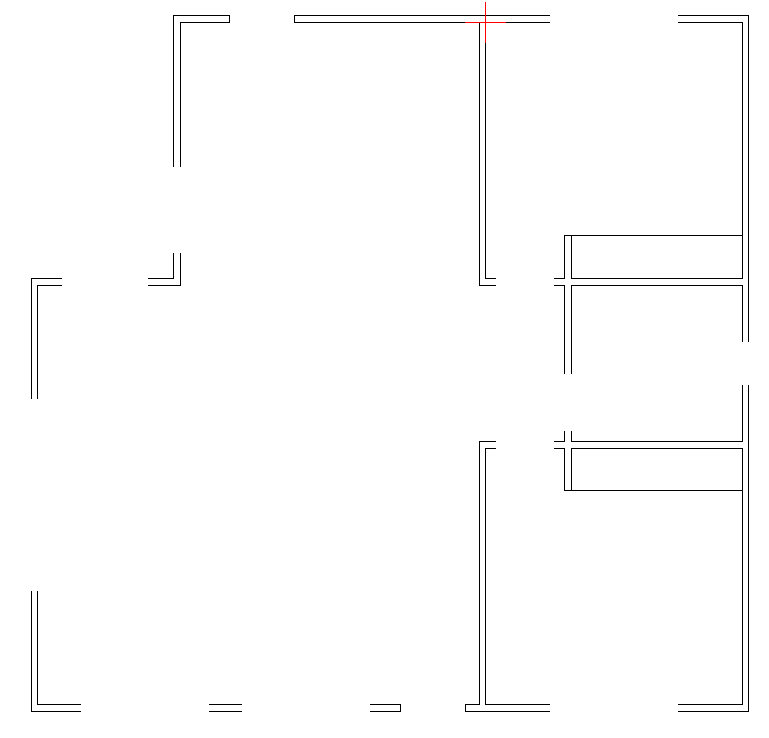
\includegraphics[width=0.75\textwidth]{figures/3_progettazione_pipeline/muri-rotti.png}
	\caption{I muri isolati risultano geometricamente incompleti: formano poligoni aperti che non rispettano le condizioni di validità imposte e richiedono una correzione.}
	\label{fig:muri_rotti}
\end{figure}

Anche le finestre presentano problemi di rappresentazione analoghi: ciascuna è composta da centinaia di segmenti, spesso sovrapposti tra loro; alcuni si estendono al di fuori della stanza, altri penetrano al suo interno.

Al termine della fase di correzione si ottiene il seguente risultato (Figura ~\ref{fig:modello_cad_finale}).
\begin{figure}[htbp]
	\centering
	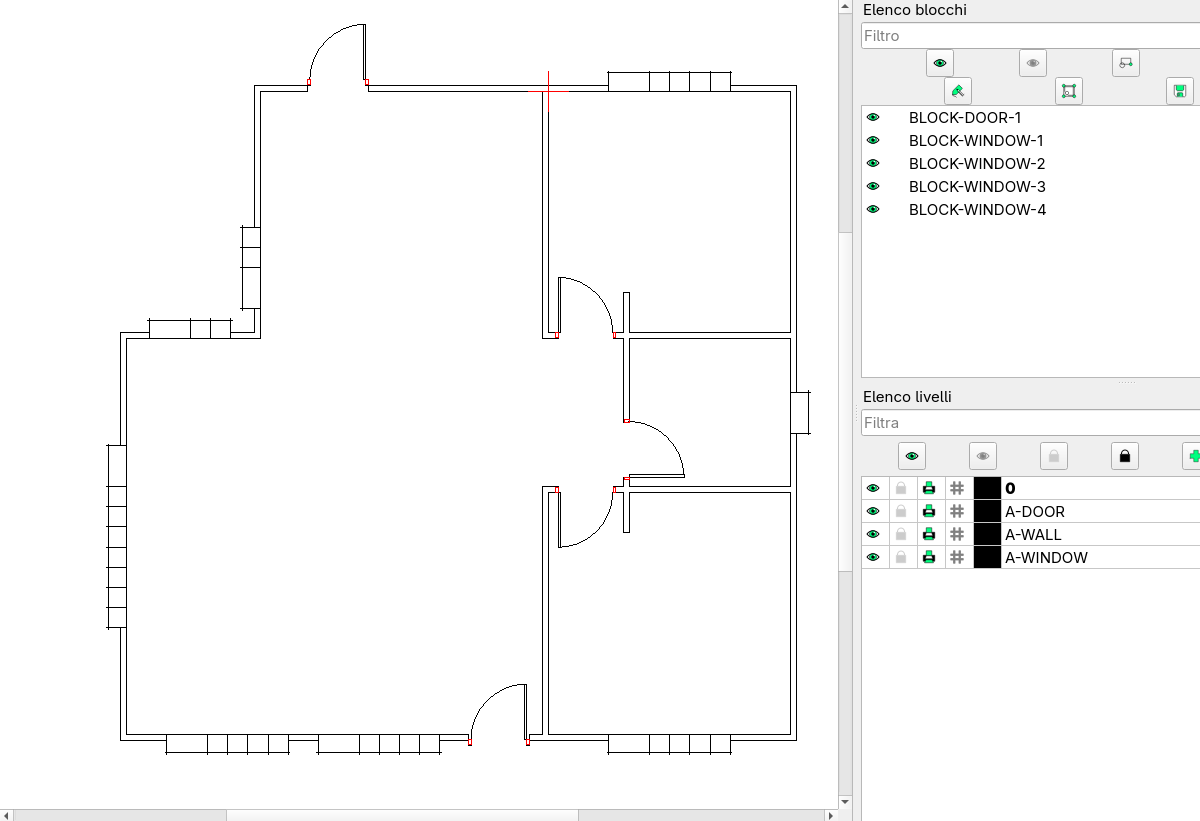
\includegraphics[width=1\textwidth]{figures/3_progettazione_pipeline/modello-cad-finale.png}
	\caption{Modello CAD al termine della fase di preprocessing: i layer e i blocchi sono stati rinominati secondo i criteri imposti, i muri esterni ridondanti sono stati rimossi e la geometria dei muri e delle finestre è stata corretta.}
	\label{fig:modello_cad_finale}
\end{figure}

